\chapter{System design}
Reader will be familiarized with architecture of our application. There are two logical parts, \textbf{public web} and \textbf{private administration}. Private administration is hidden behing \textbf{login/password}. 
\par
When designing such system, object oriented approach and grouping of similar functions together is a must. There are objects that have to be moved around the web application described in previous chapter. These objects are Post, User, Club, Cup, Position and Region. Therefore we came up with a concept of managers. Each page of SwimmPair is composed of same headerer, menu, footer. The content part is filled with page's specific results of manager call used to construct data UI page layout. These managers are included and used in all pages via \textbf{start file}.
\section{Technologies}
Following technologies are used to implement SwimmPair application:
\begin{itemize}
    \item \textbf{HTML} is HyperText Markup Language \footnote{\citep{HTML5Standard}} - application pages are templated in HTML by PHP,
    \item \textbf{CSS} is Cascading Style Sheets \footnote{\citep{CSS3Standard}},
    \item \textbf{PHP} is a general-purpose scripting language geared toward web development \footnote{\citep{PHP74Standard}} - object model and backend services are provided by it,
    \item \textbf{JavaScript}  is a general-purpose scripting language that conforms to the ECMAScript specification \footnote{\citep{ECMADocu}},
    \item \textbf{MySQL} is an open-source relational database management system \footnote{\citep{MySQLDocu}},
    \item \textbf{Git} is a distributed version control system: tracking changes in any set of files - this project is versioned and kept in public GitHub repository \footnote{\url{https://github.com/KlosStepan/SwimmPair-Www}},
    \item \textbf{Docker} is a set of platform as a service products that use OS-level virtualization to deliver software in packages called containers \footnote{\citep{DockerDocu}} - used for deployment of out application,
    \item \textbf{Kubernetes} is an open-source container orchestration system for automating software deployment, scaling, and management \footnote{\citep{K8sDocu}} - used for production deployment of our application into cluster.
\end{itemize} 
\newpage
\section{Architecture overview}
Visitor comes to \textbf{app page}, where \textbf{managers} are included. From page there are API calls on Managers that retrieve and store data data as follows.
\newline
\begin{figure}[h]	
	\centering	
    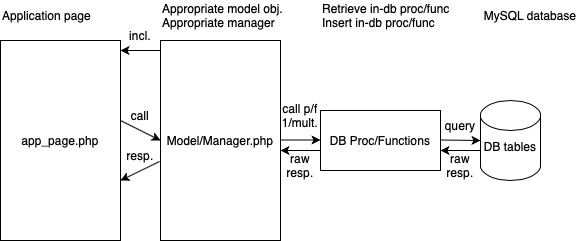
\includegraphics[scale=0.707]{img/app-schema.jpg}
	\caption{From page to manager, database, function, database and back.}
	\label{fig2.1:appschema}
\end{figure}
\section{Model Managers}
Managers are written to provide API functionality for system administration. These managers are populating pages or taking new input from them and administer process of storing them. Each object has a manager handling it and accomodates database loads and stores controlled by transactions.
\begin{itemize}
    \item Cup / CupsManager
    \item User / UsersManager
    \item Club / ClubsManager
    \item Page / PagesManager
    \item Post / PostsManager
    \item Position / PositionsManager
    \item Region / RegionsManager
\end{itemize}
Managers are implemented to extract and store data of class by which they are named after.
\newpage
\section{User Interface mockups}
In this chapter we present UI mockups of some public and private parts of our applicaton. They serve as an initial visualization mockups based on which the real UI will be made. These mockups are not 1:1 guidance, rather an idea for reader and stakeholders for the beginning.  
\subsection*{Public website mockups}
This part is concerned about displaying view-only data for public access.
\begin{figure}[h]	
	\centering	
    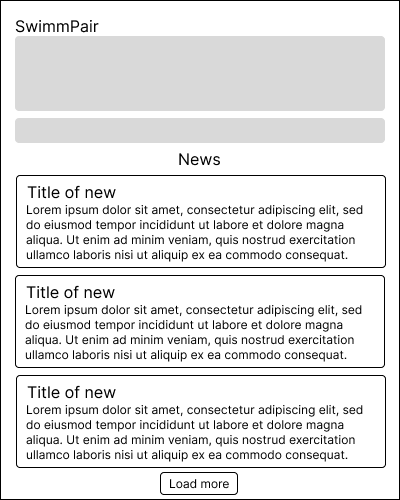
\includegraphics[scale=0.457]{img/def-U-Main.png}
    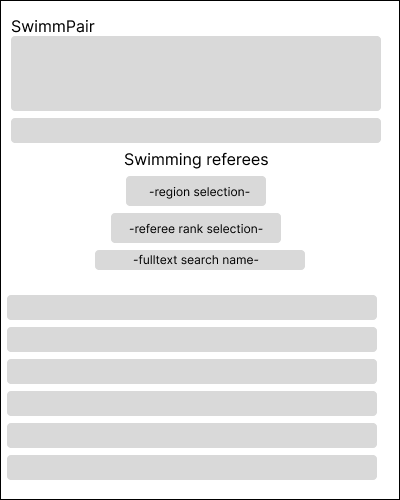
\includegraphics[scale=0.457]{img/def-U-ListingUsers.png}
    %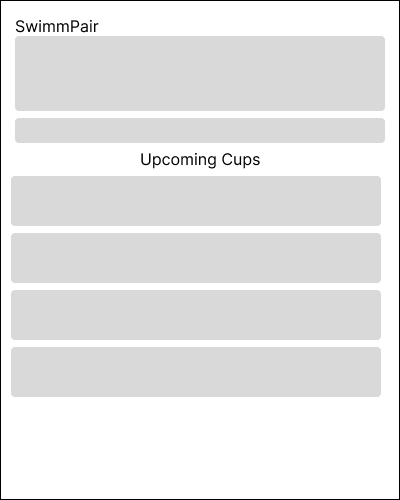
\includegraphics[scale=0.507]{img/def-U-ListingCups.png}
    %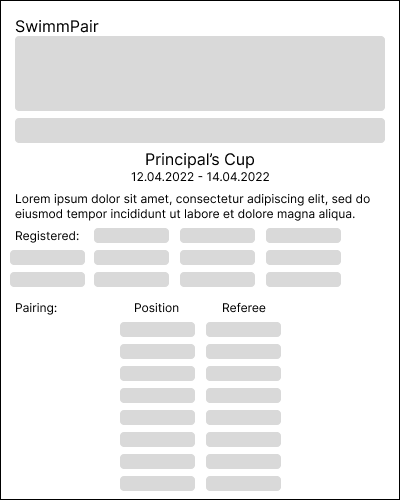
\includegraphics[scale=0.507]{img/def-U-Cup.png}
	\caption{Public pages - \underline{homepage (S5)} and \underline{listing of users (R3/S4)}.}
	\label{fig2.2:fepublicpages1}
\end{figure}
\begin{figure}[h]	
	\centering	
    %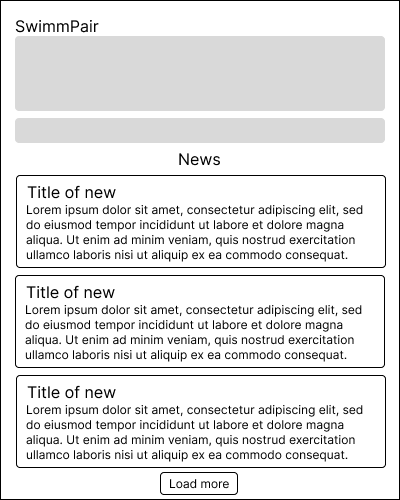
\includegraphics[scale=0.507]{img/def-U-Main.png}
    %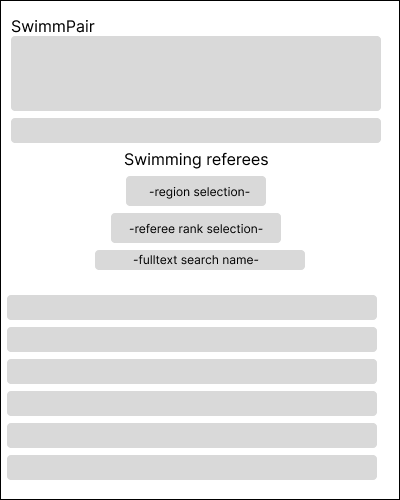
\includegraphics[scale=0.507]{img/def-U-ListingUsers.png}
    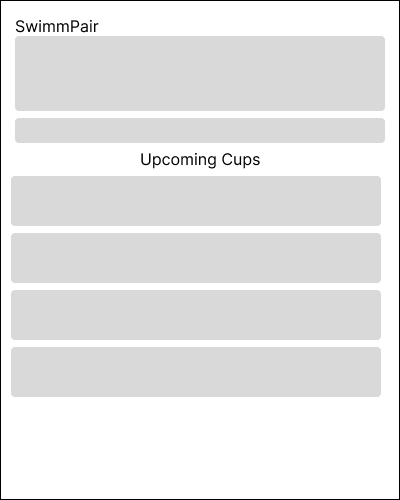
\includegraphics[scale=0.457]{img/def-U-ListingCups.png}
    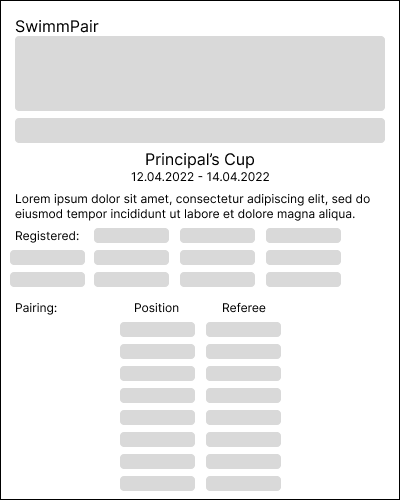
\includegraphics[scale=0.457]{img/def-U-Cup.png}
	\caption{Public pages - \underline{cups listing and cup preview (C3)}.}
	\label{fig2.3:fepublicpages2}
\end{figure}
%\newline
%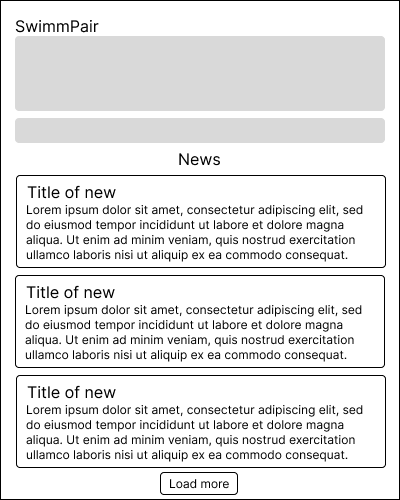
\includegraphics[scale=0.507]{img/def-U-Main.png}
%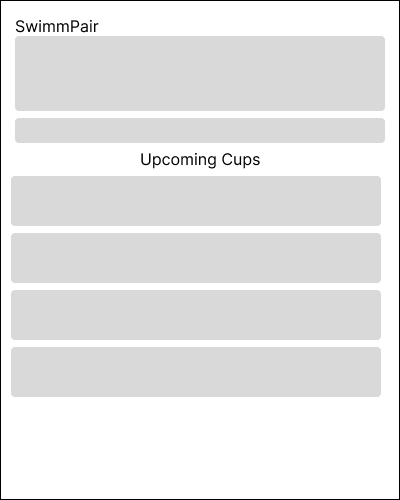
\includegraphics[scale=0.507]{img/def-U-ListingCups.png}
%\newline
%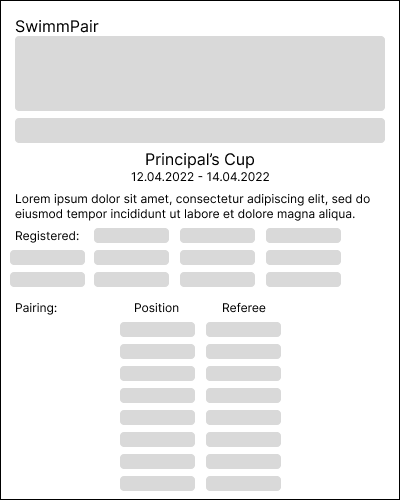
\includegraphics[scale=0.507]{img/def-U-Cup.png}
%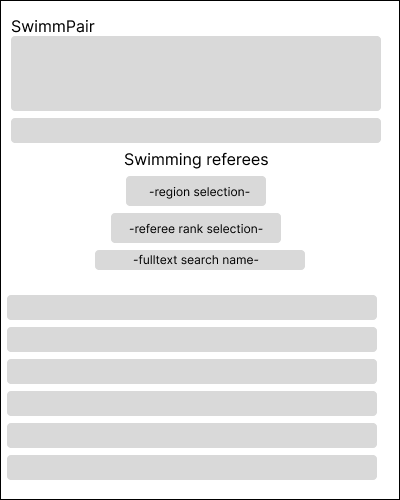
\includegraphics[scale=0.507]{img/def-U-ListingUsers.png}
\newpage
\subsection*{Administration mockups}
After logging in, user can see administrative menu. Based on rights (2/1/0) one gets layout of  appropriate sections. There is list things related to everything from administrative perspective. We will show several mockups of how functional requirements for administration can look like once programmed and designed. 
\begin{figure}[h]	
	\centering	
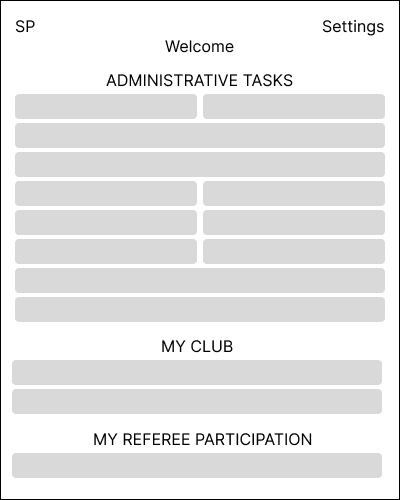
\includegraphics[scale=0.457]{img/A-administrace.png}
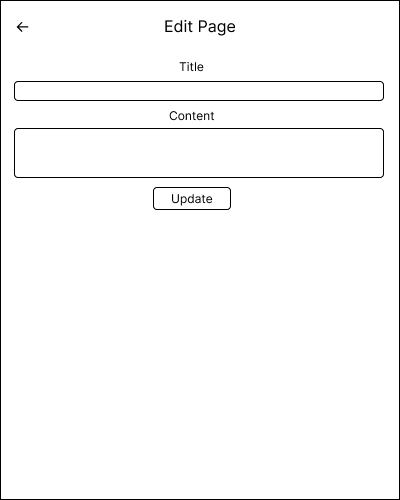
\includegraphics[scale=0.457]{img/A-edit-page.png}
\caption{Administration menu gets assembled on rights, \underline{page edit (S6)}.}
\label{fig2.4:feprivatepages1}
\end{figure}
\begin{figure}[h]	
	\centering
    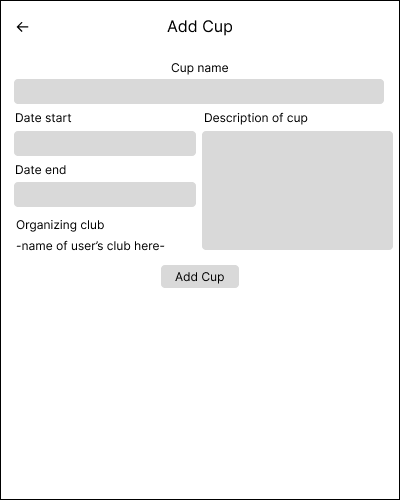
\includegraphics[scale=0.457]{img/A-new-cup.png}
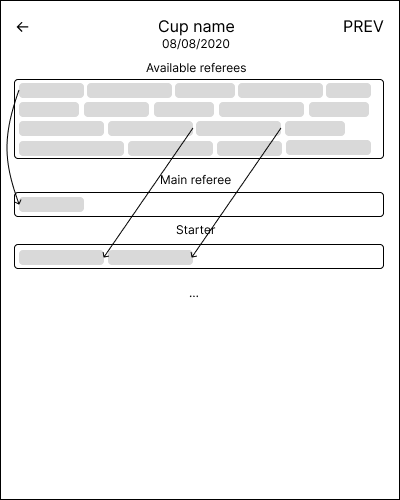
\includegraphics[scale=0.457]{img/A-pairing.png}
\caption{\underline{Add Cup (C1)} and \underline{drag'n'drop pairing (C2)}.}
\label{fig2.5:feprivatepages2}
\end{figure}
\newpage
\section{Database design}
While designing such system, well defined database schema modelled from functional requirements and entities is a necessity. Previously outlied real world (\autoref{fig1.2:uml}) has to be rigorously converted to database schema. We will show mappings and merges that had to be made in order to achieve that.
\subsection*{People entities merge}
\begin{figure}[h]	
	\centering	
    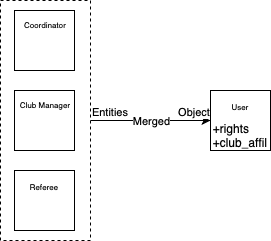
\includegraphics[scale=0.5]{img/entities_to_user.png}
	\caption{These 3 people entities got merged into the single object.}
	\label{fig2.6:enttousr}
\end{figure}
\subsection*{Pairing entities to objects}
\begin{figure}[h]	
	\centering	
    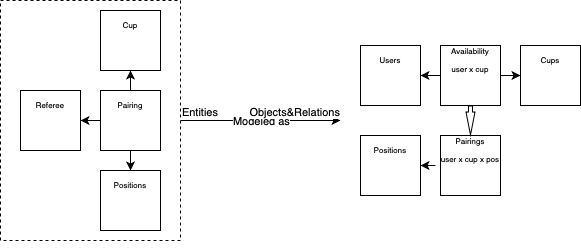
\includegraphics[scale=0.5]{img/entities_pairing_to_obj_rels.png}
	\caption{Entities modeled as 3 objects and 2 relational tables.}
	\label{fig2.7:entrels}
\end{figure}
\subsection*{Remaining entities}
Mapping of remaining entities is self-evident. 
\newpage
\subsection*{Full database schema used for out application}
\begin{figure}[h]	
	\centering	
    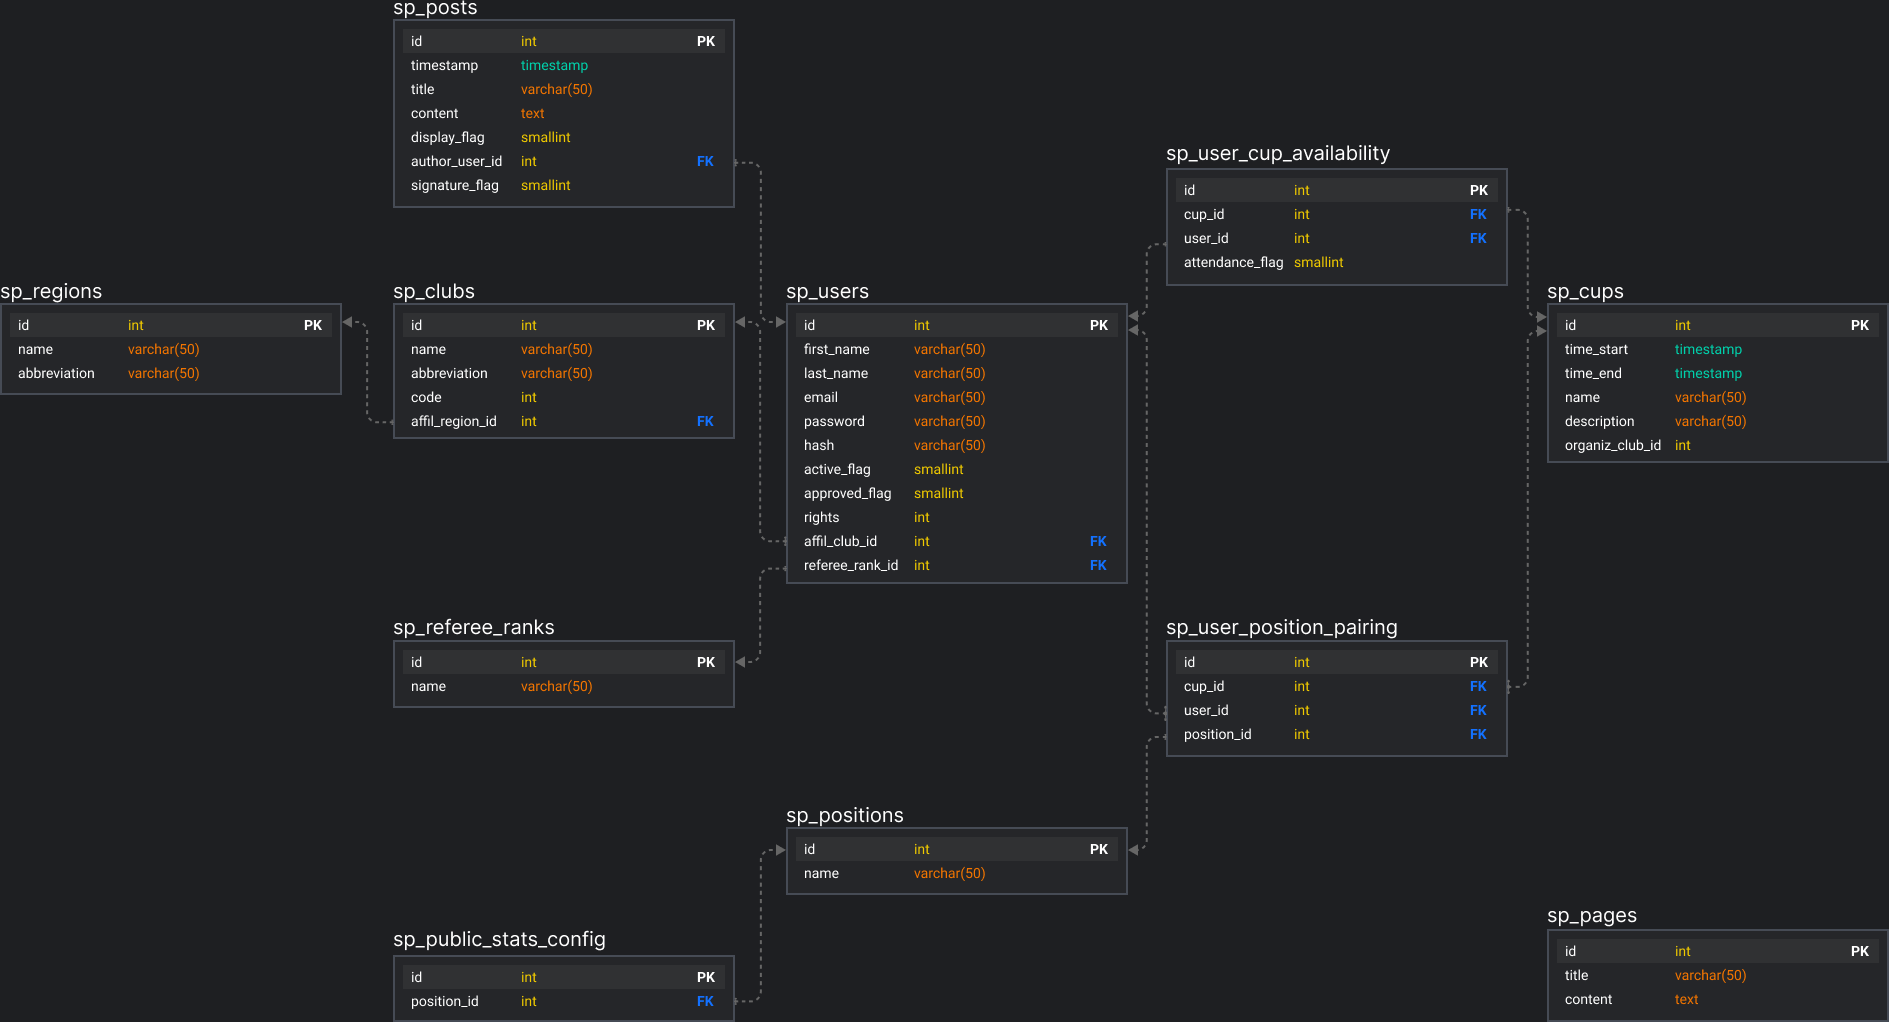
\includegraphics[scale=0.2175]{img/swimmpair_db_schema.png}
	\caption{Full database schema for the SwimmPair application.}
	\label{fig2.8:dbschemafull}
\end{figure}

\iffalse
% Let's take PostsManager as an example. This manager handles Post and is implemented as follows.
\textbf{Object - Post.php}
\begin{lstlisting}
class Post
{
    public $id;
    public $timestamp;
    public $title;
    public $content;
    public $display_flag;
    public $author_user_id;
	public $signature_flag;

    public function __construct($id, $timestamp, $title, $content, $display_flag, $author_user_id, $signature_flag)

	//7/7: {id, timestamp, title, content, display_flag, author_user_id, signature_flag}
	public function Serialize()
}

\end{lstlisting}
\textbf{Manager - PostsManager.php} 
\begin{lstlisting}
class PostsManager
{
	private $mysqli;

    //Constructor - setting $mysqli to $this->mysqli
	public function __construct(mysqli $mysqli)

    //Handling functions retrieve/store  
	public function GetPostById($id)
  	public function FindLastNPosts($N)
	public function InsertNewPost($title, $content, $display_flag, $author, $signature_flag)
    public function UpdatePost($id, $title, $content, $display_flag, $signature_flag)

    //Private functions - auxiliary controller functions
	private function _CreatePostOrNullFromStatement(mysqli_stmt $statement)
	private function _CreatePostsFromStatement(mysqli_stmt $statement)
	private function _CreatePostFromRow(array $row)
}
\end{lstlisting}
\textbf{Demonstration - public function GetPostById(\$id)}
\begin{lstlisting}
public function GetPostByID($id)
{
	$statement = $this->mysqli->prepare("CALL `GetPostById`(?);");
	$statement->bind_param('i', $id);
	return $this->_CreatePostOrNullFromStatement($statement);
}
\end{lstlisting}
Objects and their managers are made in the same manner. They contain different set of data and different number public functions. Description is included in documentation chapter below. 
\fi
\iffalse
\section{Responsive layout}
Listed media queries are used to provide design of the web by manually overriding specific classes for desired user experience outcome.
\begin{itemize}
    \item Basic CSS design
    \item @media (max-width: 768px)
    \item @media (print)
\end{itemize}
\textbf{Basic CSS design} gives definition of colors and desktop layout of our application. \textbf{Media query with max-width: 768px} supports tablets and mobile devices while \textbf{media print} of cup pairing hides redundant controll and informative elements while it keeps the pairing of cup to be printed.
\fi
\iffalse
\section{Administrative tasks}
\begin{itemize}
    \item \textbf{Add Post/Edit Post} - from PostsManager call \newline InsertNewPost/UpdatePost
    \item \textbf{Approve Newly Registered Users} - swap flag \textbf{approved} to \textbf{1}
    \item \textbf{Pair Available Users On Cup Positions} - from UsersManager call UpdatePairing - calls several SQL Procs for different things in transaction and commits/rollbacks
    \item \textbf{Add User/Edit User} - from UsersManager call AddUser/UpdateUser
    \item \textbf{Add Cup/Edit Cup} - from CupsManager call AddCup/UpdateCup
    \item \textbf{Add Club/Edit Club} - from ClubsManager call AddClub/UpdateClub
    \item \textbf{Add Region/Edit Region} - from RegionsManager call AddRegion/UpdateRegion
    \item \textbf{Configure Stats Ordering} - delete ordering, insert ordering \textbf{Nth}-\textbf{statId} 
    \item \textbf{Edit Contacts} - from PagesManager call UpdatePage
\end{itemize} 
\section{Club Manager tasks}
\begin{itemize}
    \item \textbf{Add Cup} - from CupsManager call AddCup
    \item \textbf{Sign Up People From My Club As Available For Cup} - prihlasit\_moje\_lidi\_na.php then XMLHttpRequest/call\_update\_availability.php
\end{itemize}   
\section{Referee tasks}    
\begin{itemize}
    \item \textbf{Sign Myself As Available For Cup} - add my Id to table \textbf{cupId}-\textbf{userId}
\end{itemize}
\fi
\newpage
\section {Functional requirements mapping to API}
We will show how specific \textbf{functional requirements} administrative tasks are realized via \textbf{model api functions}\footnote{\url{http://docu.swimmpair.cz/functions_func.html}}.
\newline
Table has following structure: \textbf{Task} / \textbf{Role} / \textbf{Function(s)}.
\newline
\begin{tabularx}{1.0\textwidth} { 
  | >{\raggedright\arraybackslash}X 
  | >{\centering\arraybackslash}X 
  | >{\raggedright\arraybackslash}X | }
 \hline
 Add Post & system admin& InsertNewPost \\
 \hline
 Edit Post  & system admin  & UpdatePost \\
 \hline
 Approve New Users & system admin & SetApprovedForUser \\
 \hline
 Create Pairing For Cup & system admin & DeleteOldPairing
InsertNewPairing\\
 \hline
 Add User & system admin & RegisterUser \\
 \hline
 Edit User & system admin &
 SetLoginEmailForUser
 SetRefereeRankForUser
 SetPasswordForUser\\
 \hline
 Add Club & system admin & InsertNewClub \\
 \hline
 Edit Club & system admin & UpdateClub \\
 \hline
 Add Region & system admin & InsertNewRegion \\
 \hline
 Edit Region & system admin & UpdateRegion \\
 \hline
 Configure Stats & system admin & DeleteOldStatsPositions
 InsertNewStatPosition \\
 \hline
 Edit Contacts & system admin & UpdatePage \\
 \hline
 Add Cup & club manager & InsertNewCup \\
 \hline
 Sign People From My Club Available For Cup & club manager & DeleteOldAvailability
 InsertNewAvailability \\
 \hline
 Sign Myself As Available For Cup & referee & SetAvailabilityRegister
 SetAvailabilityCantGo 
 SetAvailabilityCanGo \\
\hline
\end{tabularx}
\iffalse
These functions are used for \underline{retrieving} data to navigate across the administration.
\begin{itemize}
    \item Posts: FindAllPostsOrderByIDDesc
    \item Approve Users: FindAllInactiveUsersOrderByLastNameAsc
    \item Cups For Pairings: FindAllUpcomingCupsEarliestFirst
    \item Users: FindAllUsers
    \item Clubs: FindAllClubs
    \item Regions: FindAllRegions
    \item Stats: FindAllPositions, DisplayedLiveStatsConfiguredPositions
    \item Pages: GetPageByID
    \item Sign People From My Club Available For Cup : FindAllUpcomingCupsEarliestFirst, GetCupByID, FindAllTeamMembers, FindAllRegisteredTeamMembersForTheCup
    \item Sign Myself As Available For Cup: FindAllUpcomingCupsEarliestFirst, GetCupByID, IsUserAvailableForTheCup, IsComing
\end{itemize}
\fi